\documentclass[a4paper, 12pt]{article}

% --- CÁC GÓI THƯ VIỆN CẦN THIẾT ---
\usepackage[T5]{fontenc} % Khắc phục lỗi font tiếng Việt
\usepackage[utf8]{inputenc}
\usepackage{graphicx} % Để chèn ảnh
\usepackage{geometry} % Căn lề
\geometry{a4paper, left=2.5cm, right=2cm, top=2.5cm, bottom=2.5cm}
\usepackage{hyperref} % Tạo link mục lục
\usepackage{listings} % Chèn code
\usepackage{color}
\usepackage{float}

% Cấu hình định dạng cho code block
\definecolor{codegray}{rgb}{0.5,0.5,0.5}
\definecolor{backcolour}{rgb}{0.95,0.95,0.92}
\lstdefinestyle{mystyle}{
    backgroundcolor=\color{backcolour},   
    keywordstyle=\color{blue},
    numberstyle=\tiny\color{codegray},
    stringstyle=\color{red},
    basicstyle=\ttfamily\footnotesize,
    breakatwhitespace=false,         
    breaklines=true,                 
    captionpos=b,                    
    keepspaces=true,                 
    showspaces=false,                
    showstringspaces=false,
    showtabs=false,                  
    tabsize=2
}
\lstset{style=mystyle}

\begin{document}

\title{\textbf{Kết quả mô phỏng: Cấu hình và Mô phỏng mạng Wi-Fi trên Cisco Packet Tracer}}
\author{Made by: Tom Nguyễn}
\date{Tháng 4 năm 2026}

\maketitle

\section{Tổng quan mô hình}
Mô hình này được xây dựng để test và so sánh tốc độ thực tế của ba chuẩn Wi-Fi cũ gồm: 802.11a, 802.11b và 802.11g. Chúng ta sẽ cho các máy tính kết nối không dây, nhận IP tự động và kéo file từ máy chủ về để xem chuẩn nào chạy nhanh hơn.

Các thiết bị sử dụng trong sơ đồ:
\begin{itemize}
    \item \textbf{Router 2911:} Làm nhiệm vụ định tuyến và cấp phát IP tự động cho toàn mạng.
    \item \textbf{Switch 2960:} Làm cầu nối giữa các thiết bị có dây và điểm phát Wi-Fi.
    \item \textbf{Server:} Cung cấp trang web và nơi lưu trữ tệp tin tải xuống.
    \item \textbf{Access Point / WRT300N:} Các điểm phát sóng Wi-Fi.
    \item \textbf{Laptop:} Các máy con sẽ kết nối vào mạng để thử nghiệm.
\end{itemize}

\begin{figure}[H]
    \centering
    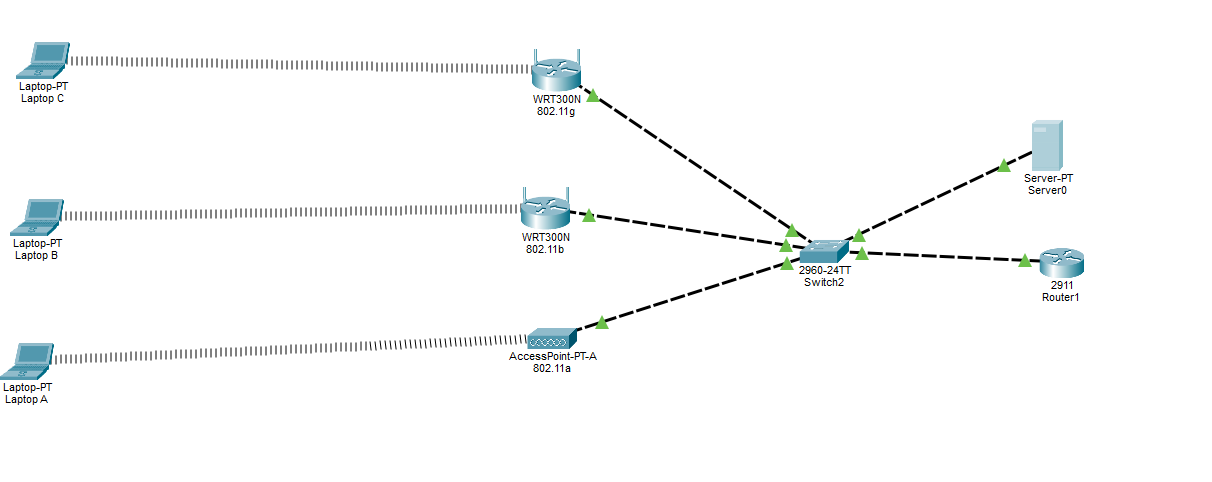
\includegraphics[width=1\textwidth]{Fig1.png}
    \caption{Sơ đồ hệ thống mạng Wi-Fi}
\end{figure}

\section{Quá trình cài đặt và Cấu hình}

\subsection{Cài đặt thiết bị phát sóng và máy con}
Với mỗi chuẩn mạng, cần lắp đúng loại card mạng cho máy con và cấu hình điểm phát tương ứng:
\begin{itemize}
    \item \textbf{Chuẩn 802.11a:} Băng tần 5GHz. Sử dụng thiết bị Access Point có đuôi chữ A. Trên Laptop, tháo card mạng dây và lắp module Wi-Fi hỗ trợ 5GHz vào.
    \item \textbf{Chuẩn 802.11b và 802.11g:} Băng tần 2.4GHz. Sử dụng bộ định tuyến WRT300N. Lưu ý quan trọng là phải \textbf{tắt tính năng DHCP tích hợp} sẵn trên WRT300N và cắm dây mạng vào cổng LAN thay vì cổng Internet. Trên Laptop, lắp module Wi-Fi phổ thông chuẩn N.
\end{itemize}

\subsection{Lập trình Router cấp phát IP tự động}
Để các Laptop nhận được IP ngay khi bắt sóng Wi-Fi, chúng ta tiến hành gõ lệnh trên Router trung tâm để tạo một vùng cấp phát IP thuộc dải mạng 192.168.1.0.

\begin{lstlisting}[language=bash, caption=Lệnh cấu hình DHCP trên Router]
Router> enable
Router# configure terminal
Router(config)# ip dhcp excluded-address 192.168.1.1 192.168.1.10
Router(config)# ip dhcp pool WIFI_POOL
Router(dhcp-config)# network 192.168.1.0 255.255.255.0
Router(dhcp-config)# default-router 192.168.1.1
Router(dhcp-config)# dns-server 192.168.1.10
Router(dhcp-config)# exit
\end{lstlisting}

\textbf{Giải thích ý nghĩa các dòng lệnh:}
\begin{itemize}
    \item \textbf{enable} và \textbf{configure terminal}: Nhóm lệnh giúp xin cấp quyền quản trị để bắt đầu cài đặt hệ thống cho Router.
    \item \textbf{ip dhcp excluded-address}: Lệnh loại trừ địa chỉ. Dặn Router giữ lại các IP từ số 1 đến số 10 để cài đặt tĩnh cho chính Router và máy chủ, tránh cấp phát nhầm cho Laptop gây trùng lặp mạng.
    \item \textbf{ip dhcp pool}: Tạo một kho chứa IP tự động và đặt tên cho nó là WIFI\_POOL.
    \item \textbf{network}: Khai báo dải mạng của kho chứa. Router sẽ lấy các IP trong dải này (đã trừ đi đoạn giữ lại ở trên) để phân phát cho các máy tính.
    \item \textbf{default-router}: Khai báo cổng cửa ngõ mặc định. Router sẽ gửi thông số IP của chính nó cho các máy tính để chúng biết đường đẩy dữ liệu ra bên ngoài.
    \item \textbf{dns-server}: Cung cấp địa chỉ máy chủ phân giải tên miền. Nhờ thông số này, các máy tính có thể truy cập trang web bằng chữ thông thường thay vì phải gõ một dãy số IP dài dòng.
\end{itemize}

\section{Các bài mô phỏng và Kết quả}

Sau khi cấu hình xong, chúng ta tiến hành 4 bài kiểm tra sau đây để đảm bảo mạng chạy ổn định và đưa ra được so sánh tốc độ.

Lưu ý quy ước về thiết bị:

\begin{itemize}
    \item \textbf{Laptop A}: chuẩn \texttt{802.11a}
    \item \textbf{Laptop B}: chuẩn \texttt{802.11b}
    \item \textbf{Laptop C}: chuẩn \texttt{802.11g}
\end{itemize}

\subsection{Kiểm tra nhận IP tự động}
Trên các máy tính, chuyển phần cài đặt mạng sang chế độ DHCP. Kết quả hiển thị thông báo thành công. Máy tính tự động nhận địa chỉ IP mới, kèm theo đúng thông số máy chủ DNS và cổng mặc định mà chúng ta đã cài trên Router.

\begin{figure}[H]
    \centering
    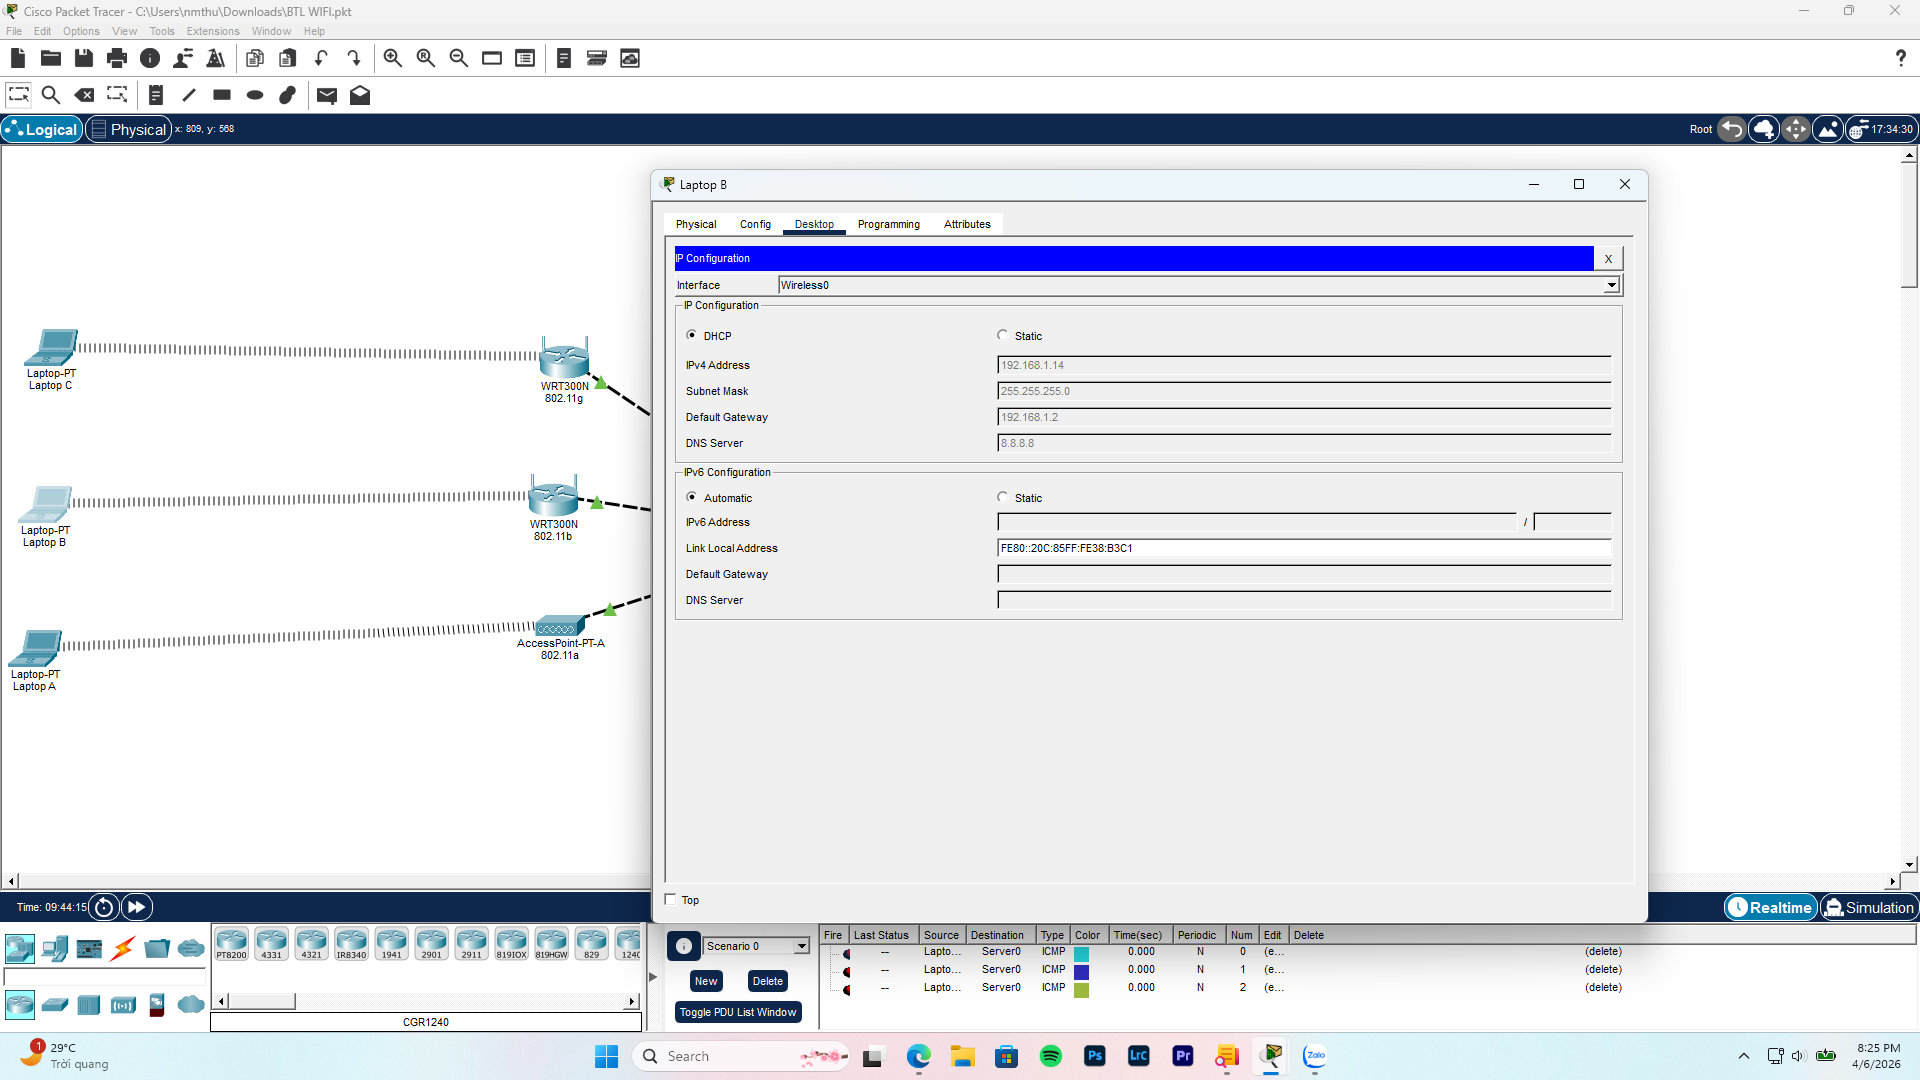
\includegraphics[width=1\textwidth]{Fig2.png}
    \caption{Máy tính nhận IP tự động thành công}
\end{figure}

\subsection{Đo độ trễ mạng bằng lệnh Ping}
Mở bảng điều khiển trên máy tính và dùng lệnh Ping để gửi các gói tin liên tục đến máy chủ. Nhìn vào kết quả thu được, chúng ta thấy một điều khá bất ngờ: độ trễ trung bình của máy dùng chuẩn 802.11b (21ms) lại ngang ngửa, thậm chí có phần nhỉnh hơn một chút so với chuẩn 802.11a (26ms) và 802.11g (28ms).

\begin{figure}[H]
    \centering
    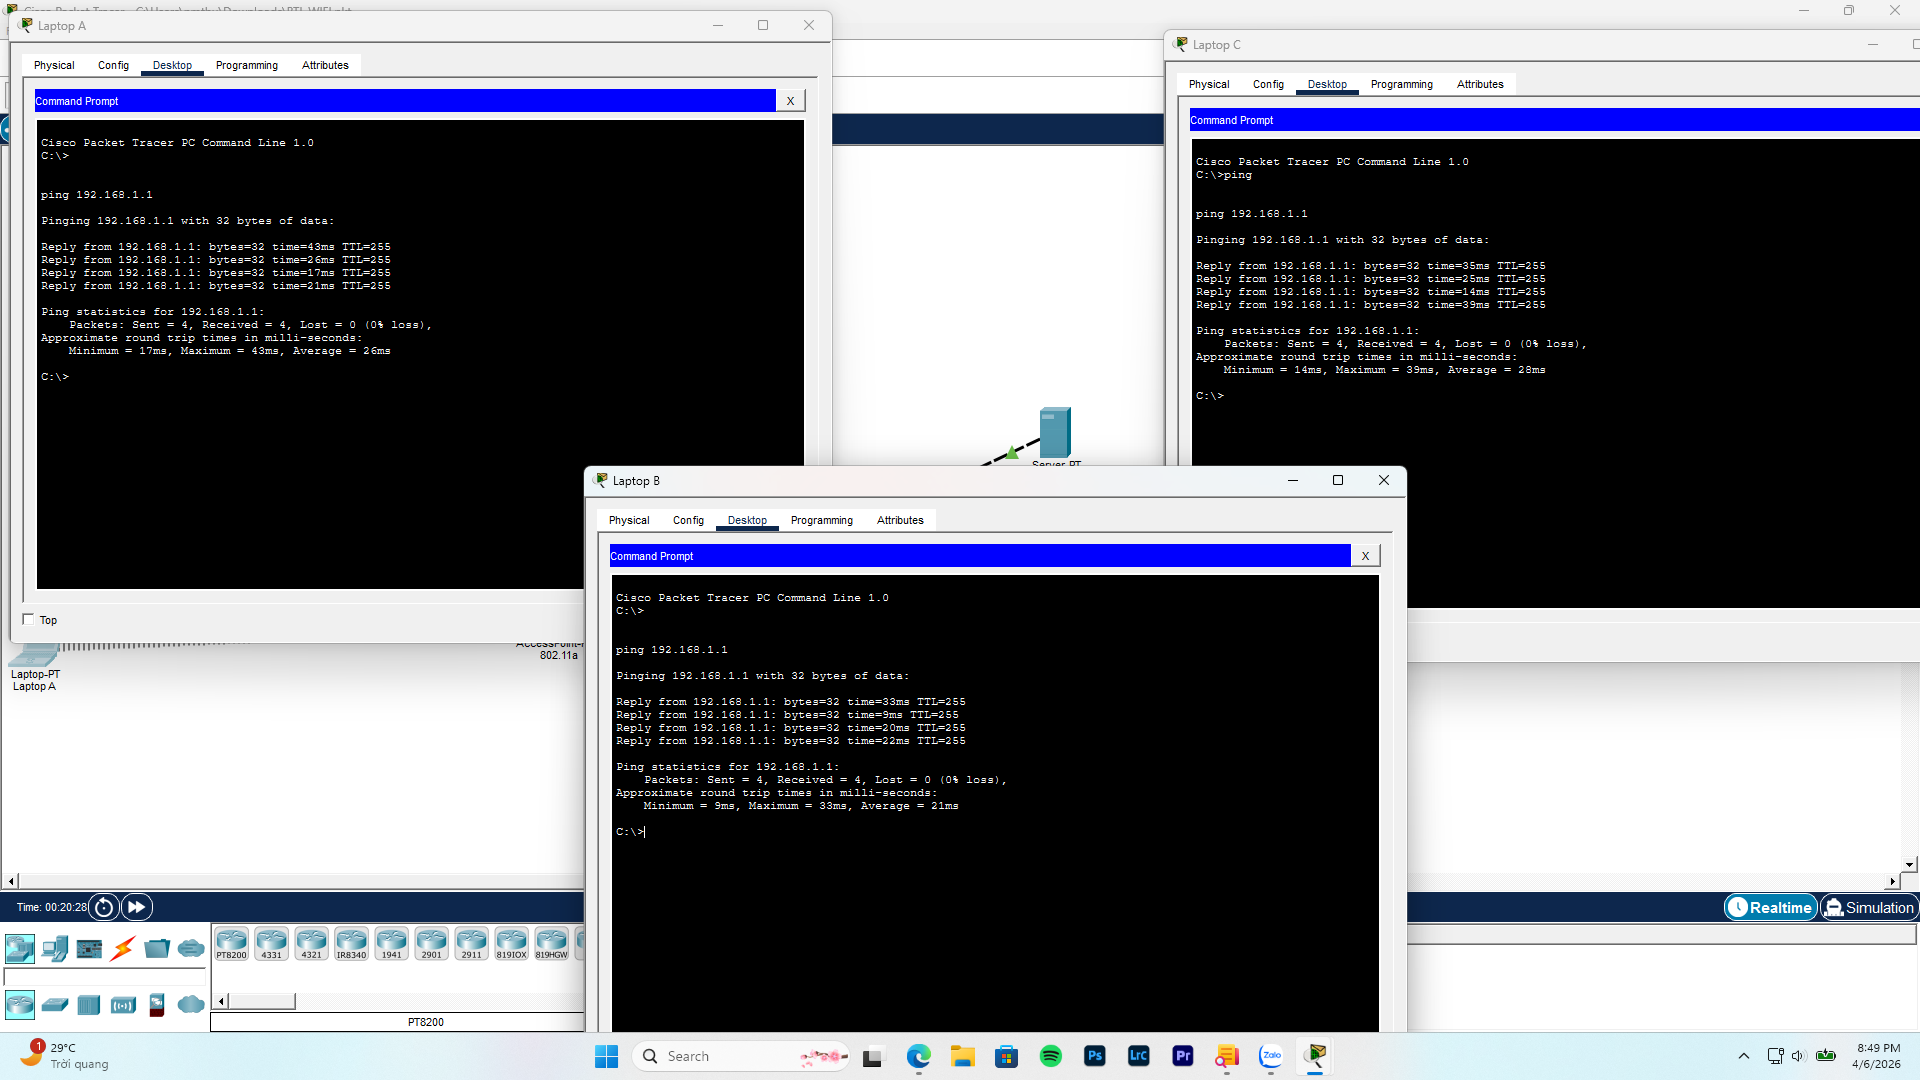
\includegraphics[width=1\textwidth]{Fig3.png}
    \caption{Sự chênh lệch về độ trễ khi Ping}
\end{figure}

\textbf{Giải thích kết quả:}
Sự thật là kết quả này hoàn toàn hợp lý với bản chất của mạng Wi-Fi vì hai lý do sau:

\begin{itemize}
\item \textbf{Kích thước gói tin quá nhỏ:} Lệnh Ping mặc định chỉ gửi đi một gói dữ liệu siêu nhẹ (chỉ 32 byte). Với dung lượng bé xíu này, dù đường truyền là 11 Megabit (chuẩn b) hay 54 Megabit (chuẩn a, g) thì cũng chỉ mất một phần ngàn giây để xử lý xong. Do đó, điểm yếu về mặt băng thông của chuẩn 802.11b không hề bị bộc lộ trong bài kiểm tra này.
\item \textbf{Cơ chế chờ ngẫu nhiên của sóng Wi-Fi:} Trước khi phát một gói tin, các thiết bị Wi-Fi luôn phải mất một khoảng thời gian ngẫu nhiên để kiểm tra xem không gian mạng có đang rảnh hay không nhằm tránh đụng độ sóng. Các con số 21ms, 26ms hay 28ms thực chất phản ánh sự chênh lệch ngẫu nhiên của thời gian chờ này và độ trễ xử lý của các thiết bị trạm, chứ không đại diện cho tốc độ mạng.
\end{itemize}

\textbf{Kết luận:} Bài kiểm tra Ping này làm rất tốt nhiệm vụ chứng minh cả 3 thiết bị với 3 chuẩn Wi-Fi khác nhau đều đã kết nối thông suốt với máy chủ. Tuy nhiên, để thấy rõ sự chênh lệch về tốc độ truyền tải, chúng ta buộc phải thực hiện các thử nghiệm tiếp theo hệ thống phải chở một khối dữ liệu lớn ở phần tải tệp tin.


\subsection{Mô phỏng truy cập trang web nội bộ}
Tại máy chủ trung tâm, bật dịch vụ HTTP và thiết lập một trang web đơn giản. Đồng thời, bật dịch vụ DNS và gắn tên miền cho địa chỉ IP của máy chủ. Từ trình duyệt web của các Laptop, gõ tên miền này vào. Kết quả trang web tải lên thành công, chứng tỏ các thiết bị đã kết nối thông suốt từ lớp vật lý lên đến tận lớp ứng dụng.

\begin{figure}[H]
    \centering
    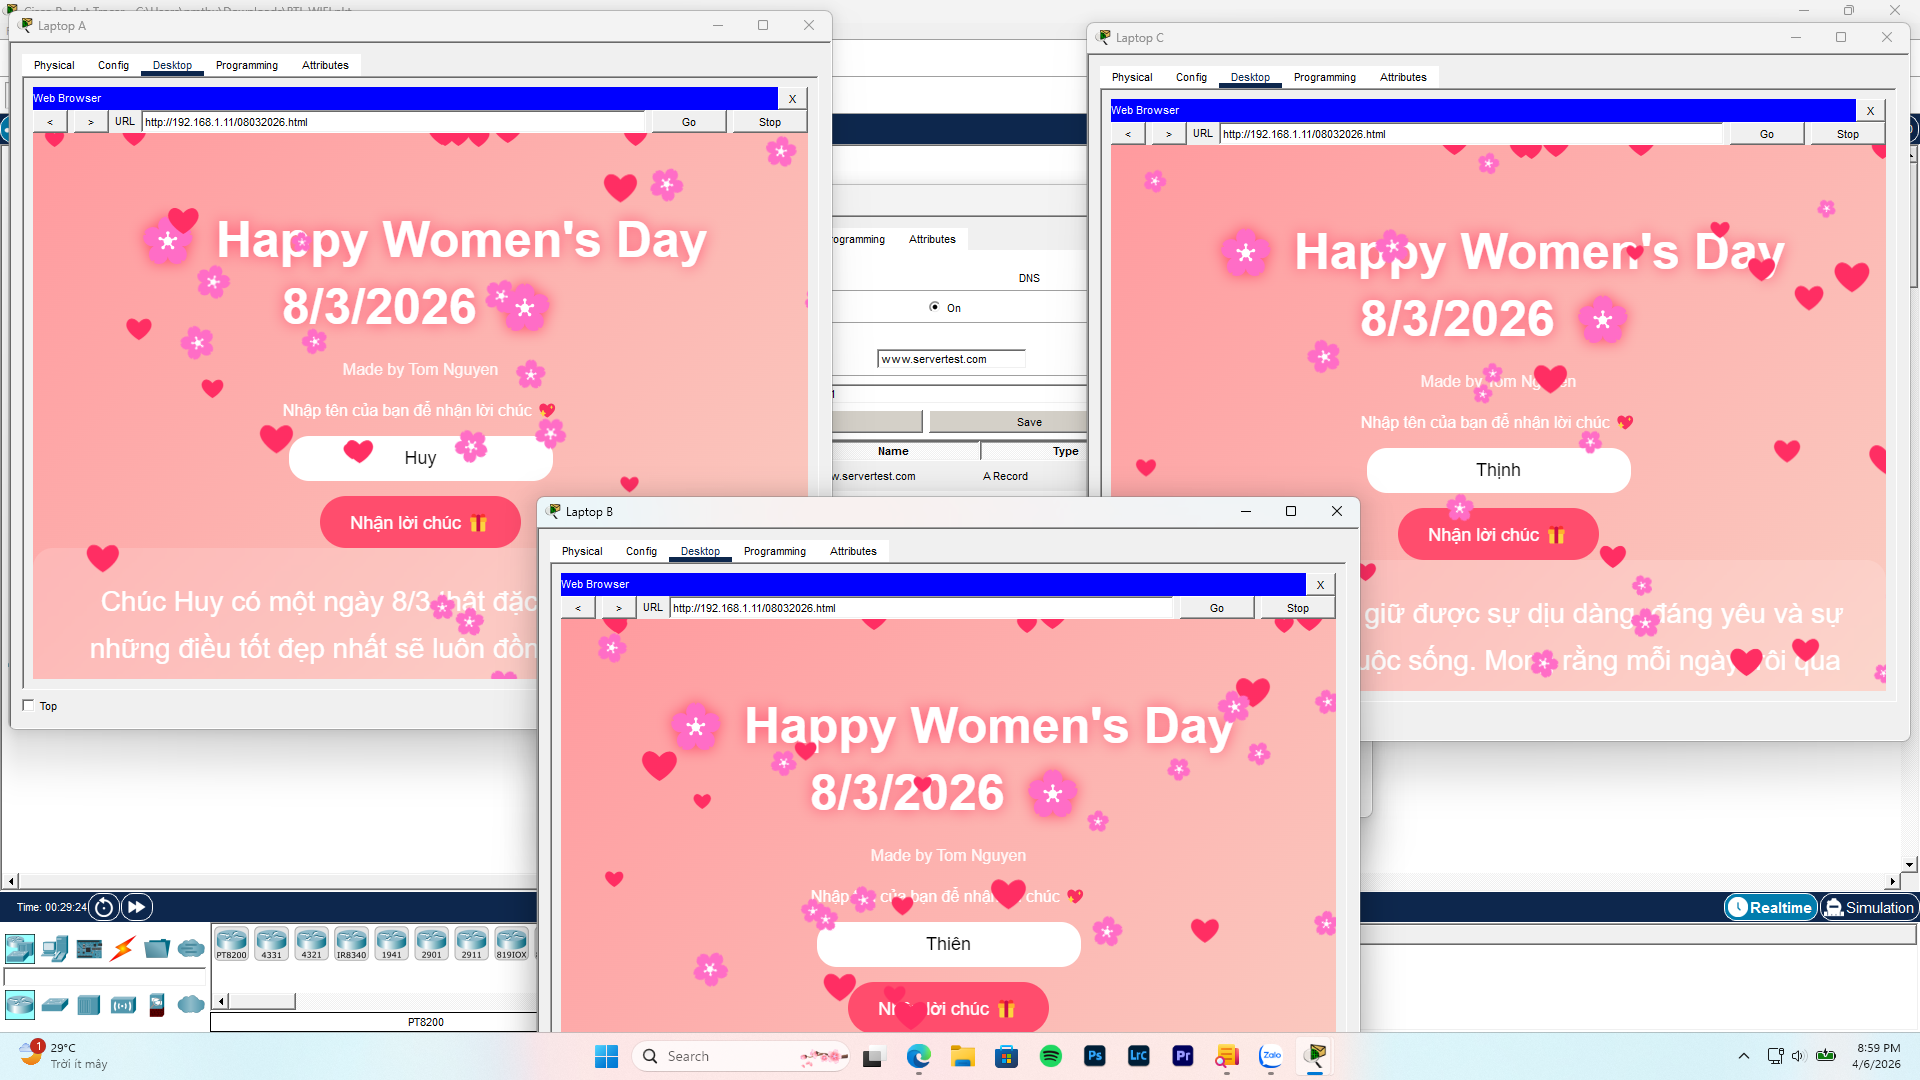
\includegraphics[width=1\textwidth]{Fig4.png}
    \caption{Truy cập trang web qua tên miền}
\end{figure}

\subsection{Kéo file dữ liệu để so sánh băng thông}
Đây là phần quan trọng nhất để xem chuẩn nào thực sự nhanh hơn. Chúng ta sử dụng một tệp tin mẫu có tên là \texttt{dumpfile1.txt} (dung lượng khoảng gần 800 KB) đặt trên máy chủ, sau đó mở chức năng FTP trên các Laptop để tải tệp tin này về và ghi nhận tốc độ.

Kết quả đo đạc thực tế từ phần mềm như sau:
\begin{itemize}
    \item \textbf{Máy dùng chuẩn 802.11a (Laptop A:} Hoàn thành trong 8.399 giây, tốc độ đạt 94.637 byte/giây.
    \item \textbf{Máy dùng chuẩn 802.11g (Laptop C):} Hoàn thành trong 10.59 giây, tốc độ đạt 75.057 byte/giây.
    \item \textbf{Máy dùng chuẩn 802.11b (Laptop B):} Hoàn thành trong 10.867 giây, tốc độ đạt 73.144 byte/giây.
\end{itemize}

\begin{figure}[H]
    \centering
    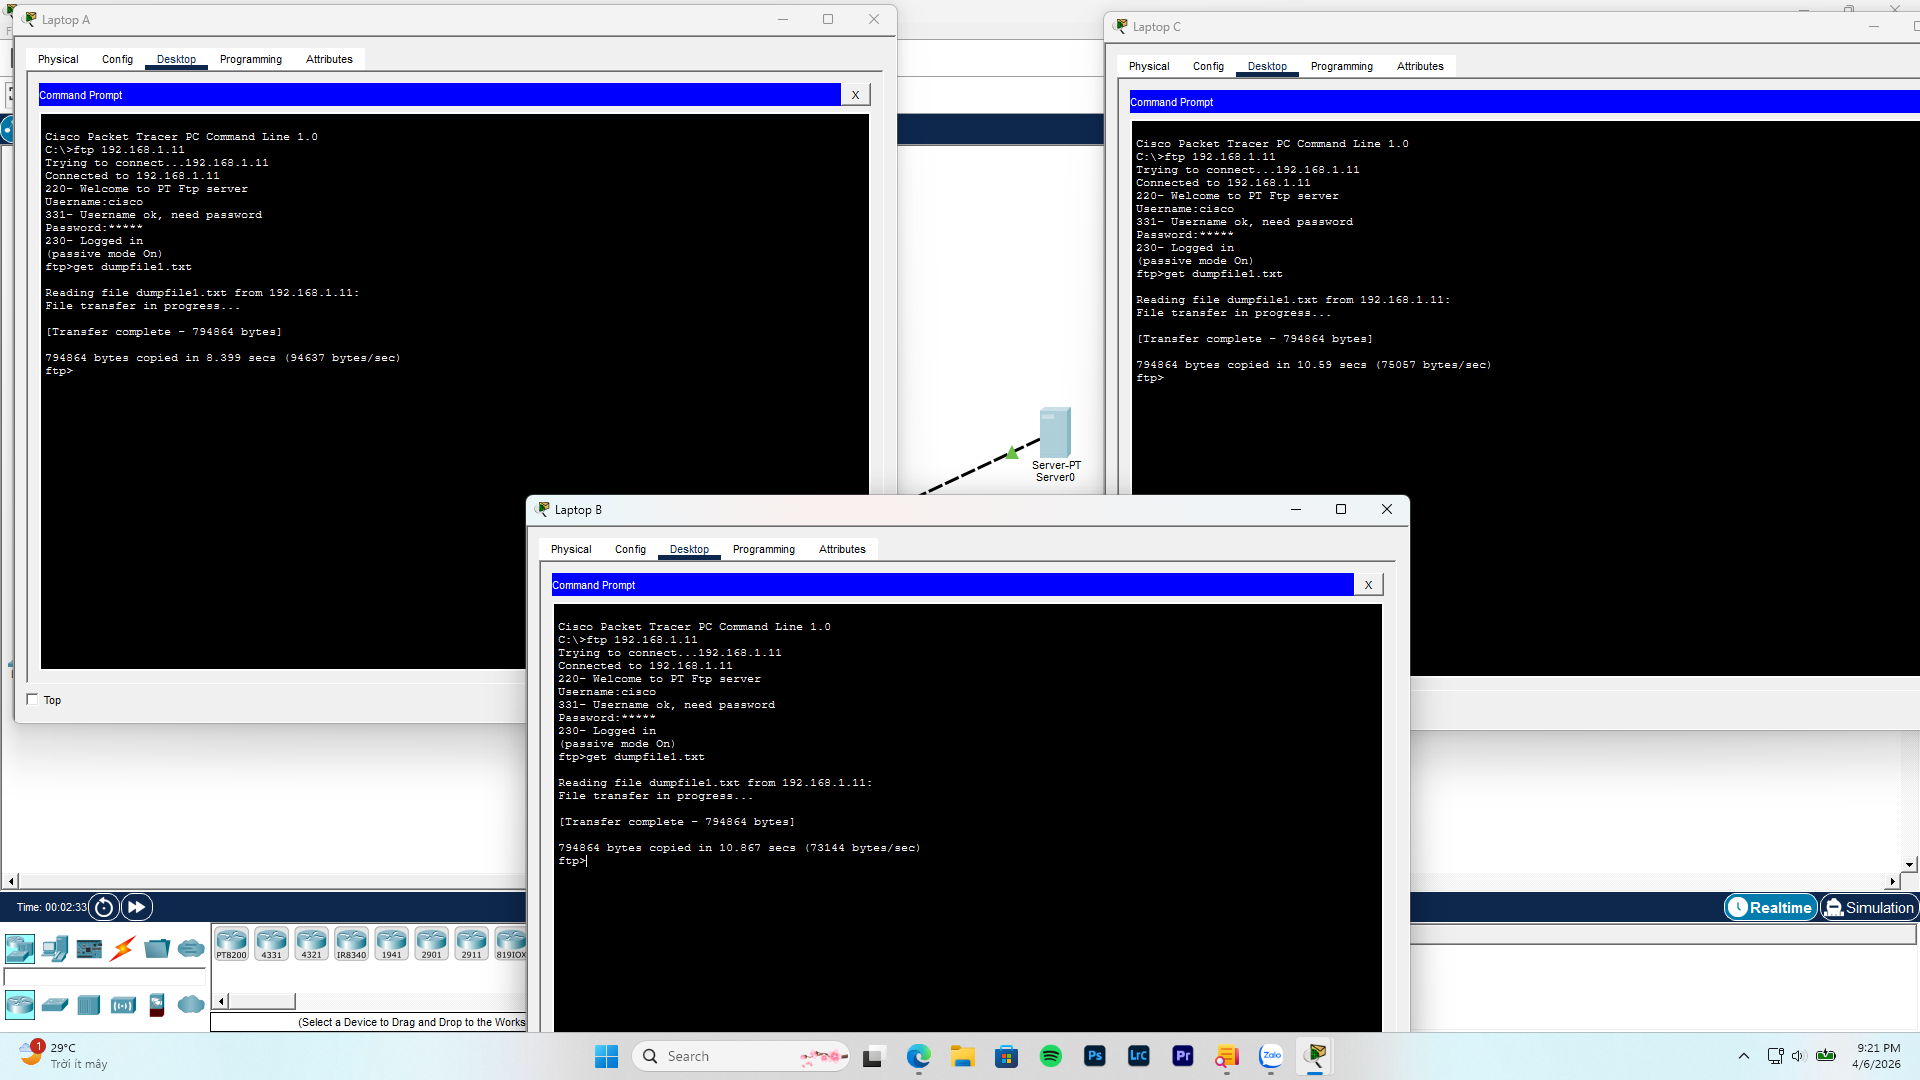
\includegraphics[width=1\textwidth]{Fig5.png}
    \caption{So sánh tốc độ tải file giữa các chuẩn Wi-Fi}
\end{figure}

\textbf{Nhận xét và Đánh giá:}

Nhìn vào các con số trên, chúng ta có thể rút ra kết luận rất thú vị về cách sóng Wi-Fi hoạt động:

\begin{itemize}
    \item Mặc dù chuẩn a và chuẩn g có cùng thông số lý thuyết là 54 Mbps, nhưng trên thực tế, chuẩn a lại cho tốc độ tải file nhanh nhất. Lý do là chuẩn a chạy trên băng tần 5GHz rộng rãi, ít bị nhiễu sóng và môi trường truyền tải thoáng hơn hẳn so với băng tần 2.4GHz.
    \item Tốc độ của hai chuẩn 802.11b và 802.11g bám khá sát nhau (quanh mức 73.000 đến 75.000 byte/giây). Nguyên nhân là do cả hai đều hoạt động chung trên băng tần 2.4GHz chật chội. Trong môi trường mô phỏng này, thời gian trễ sinh ra từ cơ chế kiểm tra để tránh đụng độ sóng đã trở thành rào cản chính, khiến chuẩn g không thể phát huy hết sức mạnh lý thuyết của nó so với chuẩn b đối với tệp dữ liệu cỡ trung bình.
\end{itemize}

\subsection{Kiểm tra độ trễ với gói dữ liệu siêu lớn (Extended Ping)}
Do hạn chế về cú pháp lệnh trên các máy tính giả lập, chúng ta sẽ sử dụng một phương pháp linh hoạt hơn: dùng tính năng Extended Ping trực tiếp từ Router trung tâm gửi đến các máy tính con. 

Bọn mình đẩy kích thước gói tin lên mức 4000 byte. Đây là một khối lượng dữ liệu lớn đối với lệnh Ping thông thường, nhằm mục đích ép phần cứng mạng phải hoạt động hết công suất.

\begin{figure}[H]
    \centering
    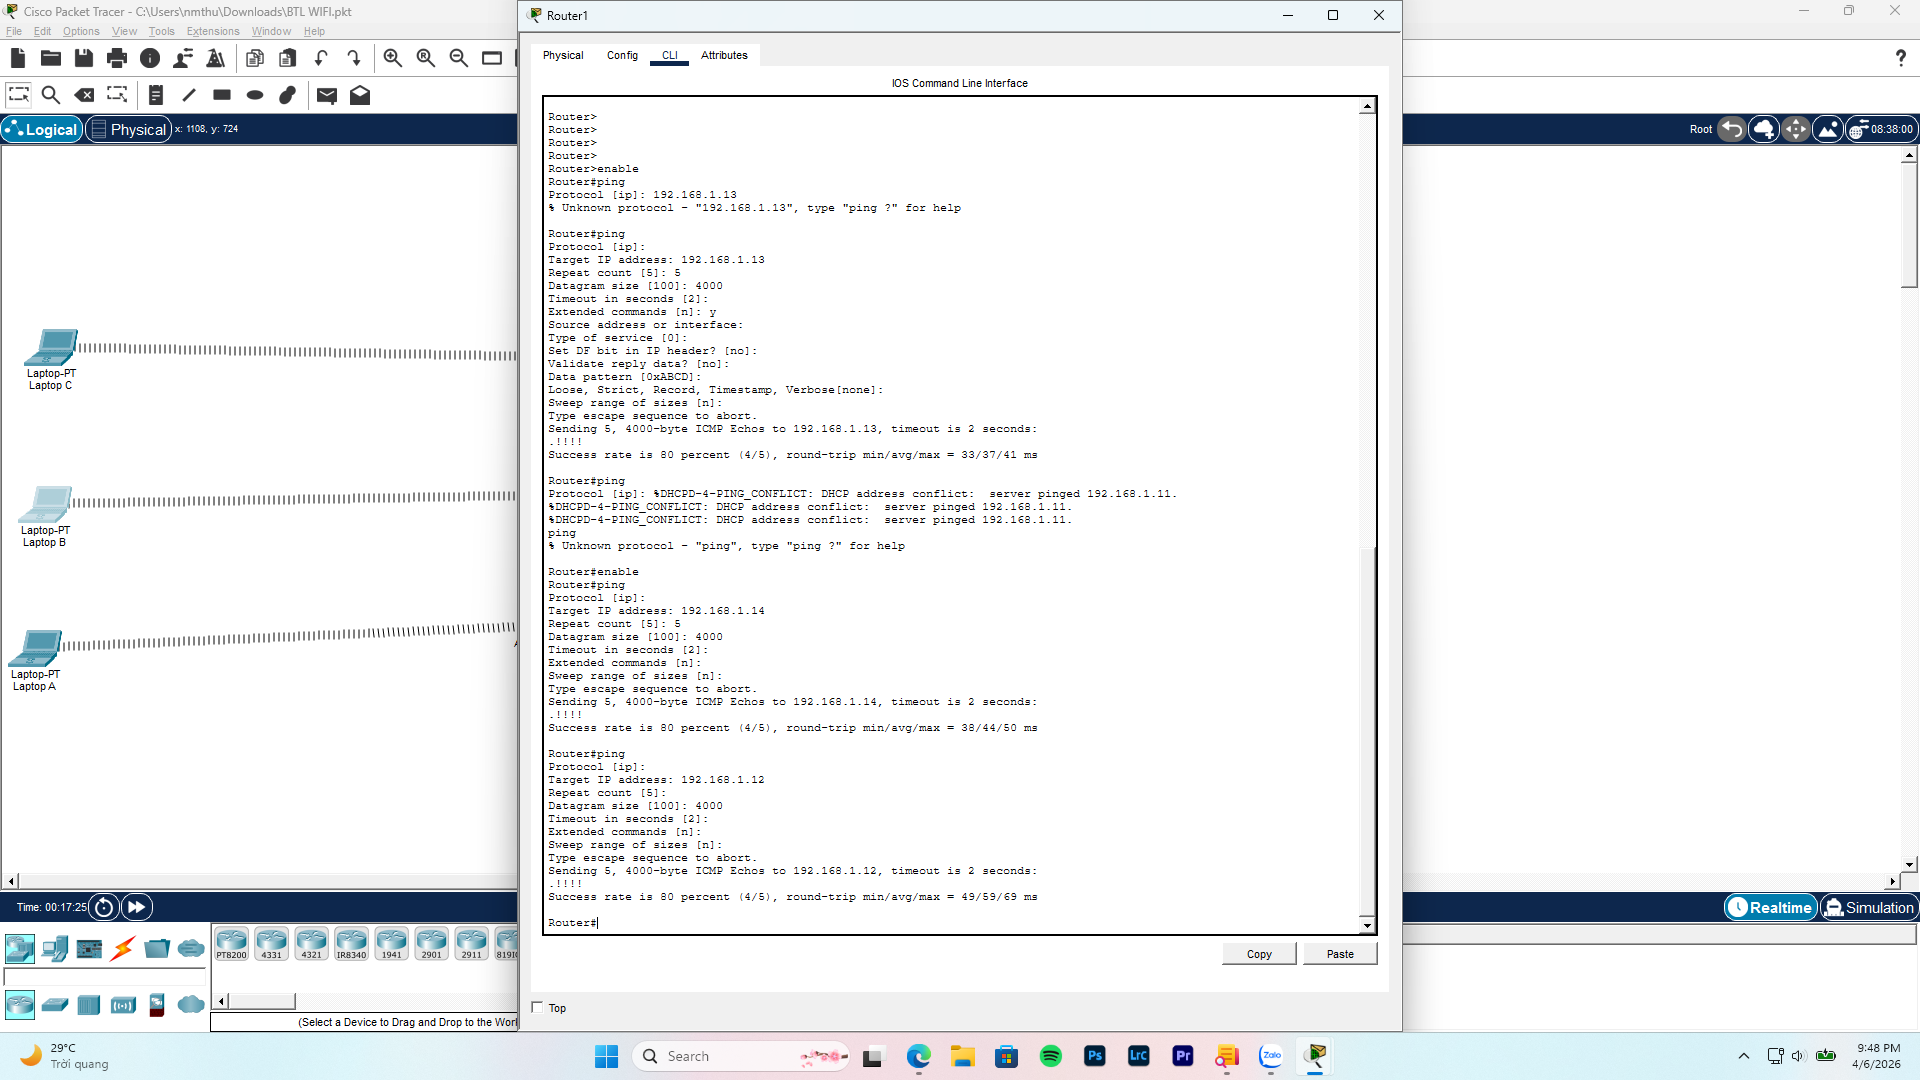
\includegraphics[width=1\textwidth]{Fig6.png}
    \caption{Đo độ trễ bằng gói tin 4000 byte từ Router đến các thiết bị}
\end{figure}

\textbf{Phân tích kết quả thực tế:}

Dựa vào bảng thông số trả về từ Router, chúng ta có thể rút ra hai hiện tượng mạng rất sát với thực tế như sau:

\textbf{1. Hiện tượng rớt gói tin đầu tiên (Tỷ lệ thành công 80\%)}
Cả 3 lượt Ping đều bị rớt mất gói tin đầu tiên. Đây không phải là lỗi mạng, mà là do bộ định tuyến cần thời gian để phát sóng tìm kiếm xem địa chỉ IP đích đang gắn với địa chỉ phần cứng MAC nào trước khi thực sự gửi dữ liệu đi. Các gói tin sau đó đều thành công.

\textbf{2. Sự chênh lệch độ trễ bất ngờ do phân mảnh dữ liệu}
Kết quả thời gian phản hồi trung bình ghi nhận được:
\begin{itemize}
    \item \textbf{Máy Laptop C (Chuẩn 802.11g - IP 192.168.1.13):} Đạt tốc độ phản hồi nhanh nhất, trung bình 37 ms.
    \item \textbf{Máy Laptop B (Chuẩn 802.11b - IP 192.168.1.14):} Tốc độ phản hồi trung bình 44 ms.
    \item \textbf{Máy Laptop A (Chuẩn 802.11a - IP 192.168.1.12):} Trễ nhất, lên tới 59 ms.
\end{itemize}

\textbf{Nhận xét:} 
Mọi người sẽ thấy hơi lạ vì sao chuẩn 802.11a băng thông cao nhất lại có độ trễ lớn nhất trong bài thử nghiệm này. Nguyên nhân là do một khung mạng tiêu chuẩn chỉ chở được tối đa khoảng 1500 byte. Khi chúng ta ép nó lên tới 4000 byte, bộ định tuyến bắt buộc phải chia gói tin này ra thành nhiều phần nhỏ để gửi đi. 

Trong môi trường mô phỏng này, thiết bị phát sóng của chuẩn 802.11a dường như mất nhiều thời gian hơn để xử lý việc điều phối các mảnh vỡ dữ liệu này so với bộ định tuyến tổng hợp của chuẩn 802.11b và 802.11g. Tuy nhiên, nhìn chung chuẩn 802.11g vẫn cho thấy sự tối ưu tốt nhất khi kết hợp được cả khả năng xử lý nhanh và độ trễ thấp ở mức 37 ms.

\subsection{Mô phỏng trực quan quá trình luân chuyển dữ liệu và phân tích độ trễ}
Thông qua tính năng mô phỏng trực quan của phần mềm, chúng ta có thể quan sát chi tiết từng bước di chuyển của các khối dữ liệu trên hệ thống mạng theo thời gian thực, từ đó bóc tách được nguyên nhân gốc rễ dẫn đến sự chênh lệch về thời gian phản hồi giữa các thế hệ mạng.

\textbf{1. Quá trình phát lệnh và truyền tải đường lên:}
\begin{itemize}
    \item Ngay khi hệ thống bắt đầu chạy mô phỏng, ba thiết bị đầu cuối đồng thời tạo ra ba khối dữ liệu kiểm tra kết nối định tuyến.
    \item Các khối dữ liệu này rời khỏi máy tính và truyền qua môi trường không khí để tiếp cận các bộ phát sóng vô tuyến tương ứng.
    \item Quan sát bằng mắt thường trên giao diện mô phỏng, chúng ta có thể nhận thấy rõ sự khác biệt về tốc độ truyền tải trên môi trường vô tuyến: khối dữ liệu phát ra từ thiết bị sử dụng chuẩn mạng 802.11b di chuyển chậm hơn đáng kể và mất nhiều thời gian hơn để chạm tới bộ phát sóng so với thiết bị sử dụng chuẩn 802.11a và 802.11g.
\end{itemize}

\textbf{2. Quá trình xử lý tại trung tâm và truyền tải đường xuống:}
\begin{itemize}
    \item Sau khi vượt qua môi trường vô tuyến, các khối dữ liệu đi vào môi trường cáp đồng tĩnh, di chuyển qua bộ chuyển mạch trung gian và hội tụ tại Máy chủ trung tâm.
    \item Máy chủ tiếp nhận, xử lý và ngay lập tức tạo ra các khối dữ liệu phản hồi, đẩy ngược trở lại đường dẫn cũ.
    \item Khi các khối dữ liệu phản hồi về đến ba bộ phát sóng vô tuyến, hiện tượng thắt cổ chai một lần nữa xuất hiện rõ rệt. Thiết bị phát sóng chuẩn 802.11b mất rất nhiều thời gian để bơm gói dữ liệu vào không gian, khiến gói dữ liệu của nó về đích muộn nhất, kéo dài tổng thời gian thực thi của cả quá trình.
\end{itemize}

\textbf{Nhận xét và Phân tích bản chất độ trễ:}
Dựa vào hình ảnh trực quan và bảng danh sách sự kiện được ghi nhận từ phần mềm, chúng ta có thể giải thích bản chất của độ trễ mạng như sau:
\begin{itemize}
    \item \textbf{Độ trễ truyền phát ở công nghệ cũ:} Nguyên nhân chính khiến gói dữ liệu của chuẩn 802.11b di chuyển chậm chạp trên màn hình là do sự hạn chế về băng thông. Với mức năng lực tối đa chỉ 11 Megabit mỗi giây, bộ phận phần cứng thu phát sóng cần nhiều thời gian hơn để chuyển đổi toàn bộ cấu trúc các hạt bit của khối dữ liệu thành tín hiệu điện từ và đẩy vào không khí. Sự chậm trễ cơ học này tích tụ ở cả chiều đi và chiều về tạo ra độ trễ lớn.
    \item \textbf{Sự tối ưu của thế hệ mới:} Ngược lại, chuẩn 802.11a và 802.11g sở hữu băng thông lên tới 54 Megabit mỗi giây. Băng thông mở rộng cho phép phần cứng "bơm" dữ liệu vào không gian với tốc độ cực nhanh, giảm thiểu tối đa thời gian khối dữ liệu phải lưu lại trên môi trường vô tuyến, từ đó mang lại tốc độ phản hồi tổng thể thấp hơn và độ ổn định cao hơn rất nhiều.
\end{itemize}

\end{document}